\PassOptionsToPackage{sols}{handout}
\documentclass[main]{subfiles}
\setcounterrefbeforedot{chapter}{m-ws2-3}
\setcounterrefafterdot{section}{m-ws2-3}
\addtocounter{section}{-1}
\usepackage{solutions}

\begin{document}

\ifSubfilesClassLoaded{%
  \chaptermark{\chaptertwo}
}{}

\section{Sinusoidal Functions} \label{ws2-3}

% \begin{objectives}

% Learning Objectives:

% \begin{itemize}[topsep=0pt,partopsep=0pt,parsep=8pt,itemsep=0pt]

% \item You should understand the definition of a ``periodic function'' and
%   the definition of its period.  You should be able to distinguish among
%   sinusoidal functions, periodic functions which are not sinusoidal, and
%   functions which are not periodic at all.

% \item You should be able to identify the midline value, amplitude, and
%   period of a sinusoidal function given its formula or graph.

% \item You should be able to graph a sinusoidal function and find
%   coordinates of important points such as local minima and maxima (without
%   using derivatives!).

% \item You should be able to write the formula for a sinusoidal function
%   given information about the period, amplitude, and midline value or
%   given its graph.

% \end{itemize}
% \end{objectives}

\textbf{Key Idea}: The graphs of the sine and cosine functions are periodic waves.

\begin{enumerate}
\item 
\begin{problem}
On your homework, you sketched the graph of the sine function. Sketch the graph again here and label the axes with appropriate variables. (Try to recall how you did it from memory!)

\begin{problemonly}

\includegraphics[scale=1.3]{tikz/2-3/2-3-axes.pdf}
\end{problemonly}
\end{problem}
\begin{solution}
    \includegraphics[scale=1.3]{tikz/2-3/2-3-axes-sine.pdf}
\end{solution}

\item 
\begin{problem}
Sketch the graph of the cosine function.

\begin{problemonly}

\includegraphics[scale=1.3]{tikz/2-3/2-3-axes.pdf}
\end{problemonly}
\end{problem}
\begin{solution}
    \includegraphics[scale=1.3]{tikz/2-3/2-3-axes-cosine.pdf}
\end{solution}

\item We say that the sine and cosine functions are \emph{periodic} because, as the input changes, the outputs eventually repeat themselves.

\begin{enumerate}
    \item
    \begin{problem}
    Explain by referring to the unit circle why the output values of sine and cosine eventually repeat.
    \end{problem}
    \pspace{\vfill}
\begin{solution}
    The functions of sine and cosine correspond to the $x$- and $y$- coordinates of an angle's terminal point location, in standard position. Every 360 degrees or $2\pi$ radians, we've completed one revolution around the circle and are now retracing the same set of positions as before, which will mean the $x$- and $y$-coordinates are repeating, since we are retracing the same positions.  
\end{solution}
    \item 
    \begin{problem}
    What is the \textbf{period} $T$ for both sine and cosine?
    \end{problem}
    
    \pspace{\vfill}
    \begin{solution}
        The period for both functions is $2\pi$. This is the angle measure we must past through to make one revolution around the circle.
    \end{solution}
    

    \item
    \begin{problem}
    How can we express using function notation that a function's values repeat every $T$ units?
    \end{problem}
    
    \pspace{\vfill}
    \begin{solution}
    $f(x) = f(x+kT)$ where $k$ is any integer. This statement means that the function value at $x$ is the same as the function achieved at $x$ plus any multiple of $T$. In this case, our period is $2\pi$, so we can make the more specific statement $f(x) = f(x+2k\pi)$ for the functions of sine and cosine.
    \end{solution}
    
\end{enumerate} 

\item 
\begin{problem}
A wave is a graph that oscillates up and down around a horizontal line, called the \textbf{midline}. The vertical distance from the midline to a peak or trough is called the \textbf{amplitude}. What are the midline and amplitude for the sine and cosine graphs?
\end{problem}
\pspace{\vfill}

\end{enumerate}

\newpage

\begin{framed}
\textbf{Sinusoidal functions}

    The term \textbf{sinusoidal function} or simply \textbf{sinusoid} is
    used to refer to the sine and cosine functions, as well as
    transformations of them obtained by shifting, reflecting, and scaling their graphs.

 The graph of any sinusoidal function has a period, amplitude, and midline.
  \begin{center}
    
\includegraphics{tikz/2-3/2-3-sinusoid.pdf}
  \end{center}

The \textbf{midline} is the horizontal line that the graph oscillates around, halfway between the peaks and troughs.

The \textbf{amplitude} is the vertical distance from the midline to a peak or a trough.

The \textbf{period} is the change in the input over one cycle, from peak to peak or trough to trough.
  
\end{framed}

\begin{enumerate}[resume]
\item

\begin{problem}
    Let's look at an example of a sinusoidal graph.
\end{problem}
  
  \setlength{\columnsep}{-10pt}
  \begin{multicols}{2}
  
  \begin{center}
    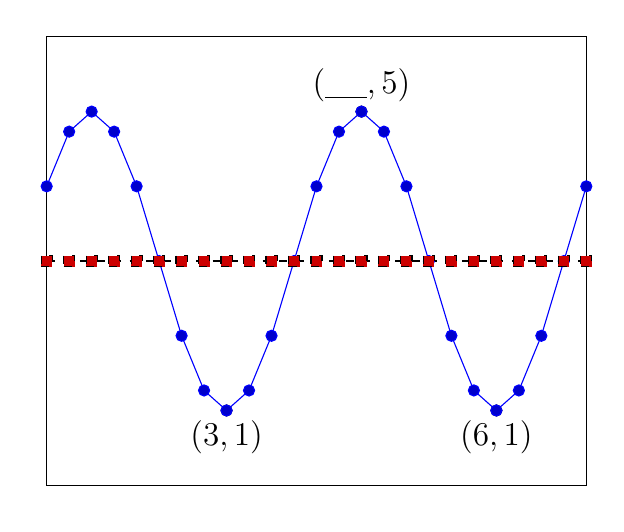
\begin{tikzpicture}
    \begin{axis}[
    axis lines = box,
    xmin = 1, xmax = 7,
    ymin = 0, ymax = 6,
    xtick distance = 1,
    ytick distance = 1,
    grid = none,
    xticklabels = \empty,
    yticklabels = \empty,
    tickwidth = 0
    ]
    \addplot+[domain=1:7]{-2*cos(deg(2*pi*x/3))+3};
    \addplot+[domain=1:7,dashed,black]{3};
    \filldraw[radius=2pt] 
    (axis cs:3,1) circle
    node[below] {\large$(3,1)$}
    (axis cs:4.5,5) circle
    node[above] {\large$(\underline{\phantom{4.5}},5)$}
    (axis cs:6,1) circle
    node[below] {\large$(6,1)$};
    \end{axis}
    \end{tikzpicture}
    \end{center}
    
    \columnbreak

    \null
    \begin{itemize}[itemsep=36pt]
    \item $\text{amplitude} = \solonly{2}$
    
    \begin{solution}
        The amplitude is the half of the vertical distance between the peaks and the troughs. $5-1 = 4$, so our amplitude is 2.
    \end{solution}
    \item midline: \solonly{$y=3$}
    
    \begin{solution}
        The midline is the horizontal line that cuts through the center of the function. Its $y$-value is the amplitude away from the peaks or the troughs. We can find this by subtracting our amplitude from the $y-$value of the peak. $5-2=3$, so our midline is $y=3$.
    \end{solution}
    \item $\text{period}= \solonly{3}$
    
    \begin{solution}
        The period is the length of the input interval before the function begins to repeat. We can find this by determining the horizontal distance between consecutive peaks or valleys. $6-3=3$. The period is 3.
    \end{solution}
    \end{itemize}
    
  \end{multicols}
  \setlength{\columnsep}{10pt}

\begin{problem}
  Given the maximum and minimum values of a sinusoidal function, how can you determine the midline and amplitude of its graph?
\end{problem}
\pspace{\vfill}

  \begin{solution} The amplitude is the half of the vertical distance between the peaks and the troughs. Compute the vertical distance between one peak and one trough and divide this distance in half.\\
  The midline is the amplitude subtracted from the $y$-value of a peak or added to the $y$-value of a trough.
  \end{solution}
\item 
\begin{problem}
    Look back at the graphs of sine and cosine. They have the exact same period, midline, and amplitude! How are the graphs different? Can you transform one into the other?
\end{problem}

\pspace{\vfill}
\begin{solution}
    We can see that the peak that occurs at $x=0$ in the cosine function, occurs at $x=\frac{\pi}{2}$ in the sine function. This visually looks like the cosine function is shifted to the right by $\pi/2$ to achieve the sine function. 
    $\cos(x-\pi/2)=\sin x$. \\
    We could also say that the sine function is shifted to the left by $\pi/2$ to achieve the cosine function, which can be written as $\sin(x+\pi/2)=\cos x$.
\end{solution}

\end{enumerate}

\pspace{\newpage}


\begin{enumerate}[resume]

\item

    The equation $y=3\sin(2t)-1$ produces a sinusoidal graph. Let's figure out what it looks like using transformations.
\begin{enumerate}
\item 
\begin{problem}
What is the parent function? What transformations should we apply to the graph? In what order?
\end{problem}
\pspace{\vfill}
\begin{solution} The parent function is $\sin t$. We first compress horizontally by a factor of 2 to get $\sin(2t)$, then we stretch vertically by a factor of 3 to get $3\sin(2t)$, then we vertically shit downward by 1 to get $3\sin(2t)-1$.
\end{solution}
\item 
\begin{problem}
Using the transformations, determine the period, amplitude, and midline of the final graph. 
\end{problem}
\pspace{\vfill}
\begin{solution}
    The period is impacted only by the horizontal compression by a factor of 2. Because $t$ is multiplied by 2 before being inputted into the sine function, it only needs to be half as large to achieve the same output. This means our period will be $\pi$.\\
    The amplitude is only impacted by the vertical stretch. The multiplication by 3 means our amplitude is 3.\\
    The midline is only impacted by the vertical shift. Our midline now sits at $y=-1$.
\end{solution}

\item
\begin{problem}
Determine the \textbf{phase} at $t=0$. What should be happening on the graph at $t=0$? Is the graph at a peak, at a trough, increasing through the midline, or decreasing through the midline?
\end{problem}

\pspace{\vfill}
\begin{solution} 
The sine function is not shifted horizontally, nor reflected over an axis, so our function will have the same phase as our parent function. $\sin t$ is increasing through the midline at $t=0$ and that's what our function will be doing too.
\end{solution}

\item
\begin{problem}
Using all of this information, sketch two periods of the graph. Make sure to hit the key points: peaks, troughs, and midline intersections. You can check your graph by plotting points.
\end{problem}

\pspace{\stretch{2}}
\begin{solution}
    \includegraphics[scale=1.3]{tikz/2-3/2-3-3sine2tminus1.pdf}
\end{solution}

\end{enumerate}
\item Graph each. Label the midline, 
   a local minimum, and a local maximum. 
  
  \note{Even when students recognize the basic shifts and stretches here,
    they often have trouble producing an accurate graph and identifying
    coordinates of key points such as local minima.

    If they are having trouble graphing, you may find the applet
    \url{http://tube.geogebra.org/student/m157623} helpful for showing
    them what's happening when you shift and stretch.  }



  \begin{enumerate}
  \item 
    \begin{problem}[\vfill]
      $y = \sin( \frac{1}{2} t)$
    \end{problem}

    \begin{solution}
      This is a horizontal stretch of $y = \sin x$ by a factor of 2 (so
      that everything is twice as wide as before).  If you can't
        remember whether it's a horizontal stretch that makes everything
        twice as wide or half as wide, try testing a few points, like you
        did in {{{Problem Set 7}, {{\#5}}}}.  
      \begin{center}
        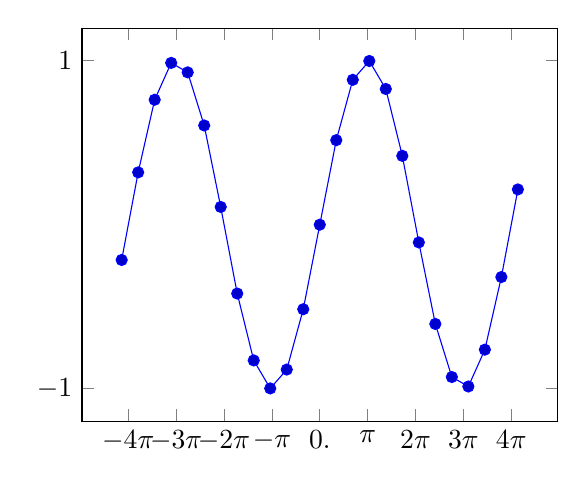
\begin{tikzpicture}
          \begin{axis}[xtick={-12.5664, -9.42478, -6.28319, -3.14159, 0.,
              3.14159, 6.28319, 9.42478, 12.5664},xticklabels={$-4 \pi$,
              $-3 \pi$, $-2 \pi$, $-\pi$, $0.$, $\pi$, $2 \pi$, $3 \pi$,
              $4 \pi$}, ytick={-1, 1}, width=3in]
            \addplot+[domain=-13:13]{sin(deg(x)/2)};
          \end{axis}
        \end{tikzpicture}      
      \end{center}

    \end{solution}

  \item
    \begin{problem}[\vfill]
      $\displaystyle y = 4 \cos(3t) - 5$
    \end{problem}

    \begin{solution}
      We can get this graph by starting with $\cos x$, doing a horizontal
      stretch by $\frac{1}{3}$ to get \color{red} $y =
      \cos(3x)$\color{black}, a vertical stretch by $4$ to get
      \color{green!70!black} $y = 4 \cos(3x)$\color{black}, and a
      shift down by $5$ to get \color{blue} $y = 4 \cos(3x) -5$\color{black}:
      \begin{center}
        \answer{
          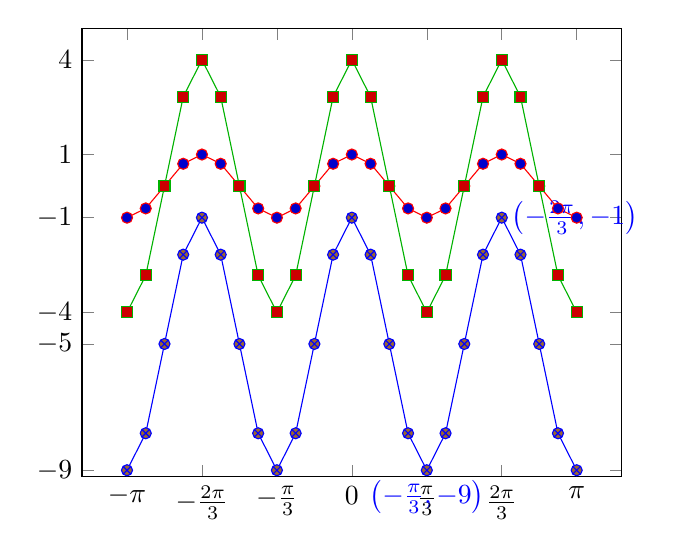
\begin{tikzpicture}
            \begin{axis}[xtick={-3.14159, -2.0944, ..., 3.14159},
              xticklabels={$-\pi$, $-\frac{2\pi}{3}$, $-\frac{\pi}{3}$, $0$,
                $\frac{\pi}{3}$, $\frac{2\pi}{3}$, $\pi$},
              ytick={-4, 4, -1, 1, -5, -9}, ymin=-9.2, ymax=5, clip=false]
              \addplot+[domain=-pi:pi, red]{cos(deg(3*x))};
              \addplot+[domain=-pi:pi, green!70!black]{4*cos(deg(3*x))};
              \addplot+[domain=-pi:pi, blue]{4*cos(deg(3*x))-5};
                \filldraw[blue] (axis cs: 1.05, -9) circle(1.5pt) node[below]
                {$\left( - \frac{\pi}{3}, -9 \right)$};
                \filldraw[blue] (axis cs: 2.1, -1) circle(1.5pt) node[right]
                {$\left( - \frac{2 \pi}{3}, -1 \right)$};
            \end{axis}
          \end{tikzpicture}
        }
      \end{center}
      The horizontal stretch by $\frac{1}{3}$ makes the \fbox{period
        $\frac{2 \pi}{3}$}, the vertical stretch by 4 makes the
      \fbox{amplitude 4}, and the shift down by $5$ makes the
      \fbox{midline value $-5$}. 
    \end{solution}

  \item
    \begin{problem}[\vfill]
      $ y = - 2 \sin( t - \frac{\pi}{4} )$
    \end{problem}

    \begin{solution}
      Let's first graph \color{red} $y = \sin \left( x - \frac{\pi}{4}
      \right)$ \color{black}, since we know that \color{blue} $y = - 2 \sin
      \left( x - \frac{\pi}{4} \right)$ \color{black} is then just a
      vertical flip and stretch of that of that.

      You should recognize that \color{red} $y = \sin \left( x -
        \frac{\pi}{4} \right)$ \color{black} is a horizontal shift of $y =
      \sin x$ by $\frac{\pi}{4}$, but it's often difficult to remember
      whether it's a shift to the right or to the left.  Rather than
      trying to commit this to memory, the easiest thing is to check a
      point.  As an example, we can see that $y = \sin \left( x -
        \frac{\pi}{4} \right)$ is 0 if we plug in $x = \frac{\pi}{4}$, so
      $y = \sin \left( x - \frac{\pi}{4} \right)$ crosses the $x$-axis at
      $x = \frac{\pi}{4}$.  This means that it must be $y = \sin x$
      shifted to the right (if you shifted $y = \sin x$ to the left, the
      graph wouldn't cross the $x$-axis at $x = \frac{\pi}{4}$). 

      \begin{center}
        \answer{
          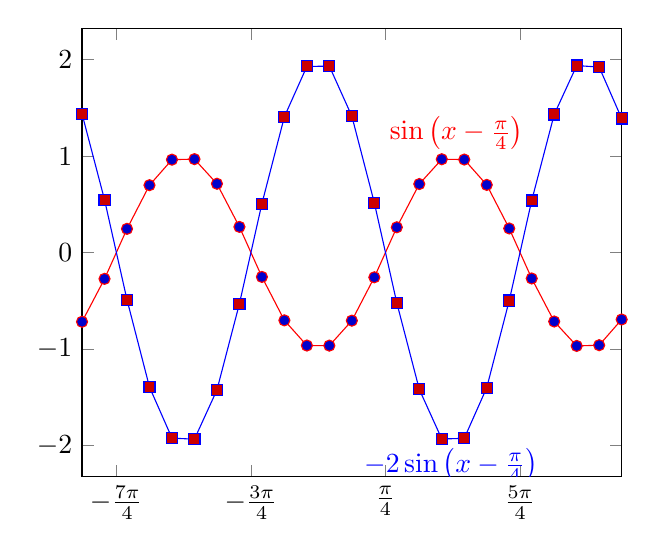
\begin{tikzpicture}
            \begin{axis}[xmin=-6.3, xmax=6.3, xtick={-5.49779, -2.35619,
                0.785398, 3.92699}, xticklabels={$-\frac{7 \pi}{4}$, $-\frac{3
                  \pi}{4}$, $\frac{\pi}{4}$, $\frac{5 \pi}{4}$}]
              \addplot+[domain=-6.3:6.3, red] {sin(deg(x-pi/4))}
              node[pos=0.7, above] {$\sin
                \left( x - \frac{\pi}{4} \right)$};
              \addplot+[domain=-6.3:6.3, blue, solid] {-2*sin(deg(x-pi/4))}
              node[pos=0.7, below] {$-2 \sin 
                \left( x - \frac{\pi}{4} \right)$};
            \end{axis}
          \end{tikzpicture}
        }
      \end{center}
      Nothing we did changed the period, so the graph has \fbox{period $2
        \pi$}.  There was a vertical stretch by 2, which makes the
      \fbox{amplitude 2}.  We didn't move the graph up or down, so it
      still has \fbox{midline value 0}. 
    \end{solution}

  \end{enumerate}

  \begin{framed}
    \textbf{Summary.} For a sinusoid of the form $y = A \sin (Bt) + C$
    or $y = A \cos (Bt) + C$:
    
    \vspace{6pt}
    Amplitude: \fitb{0.75in}{$\bm{|A|}$} \hspace{0.25in}
    Midline: \fitb{0.75in}{$y=\bm{C}$} \hspace{0.25in}
    Period: \fitb{0.75in}{$\bm{\displaystyle
        \frac{2\pi}{|B|}}$}
  \end{framed}

\end{enumerate}

\newpage

\textbf{Key Idea}: Sinusoidal functions can be used to model circular motion.

\begin{enumerate}[resume]

\item 

  The most popular paid tourist attraction in the U.K. is the London Eye,
  a giant Ferris wheel located on the bank of the River Thames in London.
  The entire structure is 135 meters tall, and the wheel has a diameter of
  120 meters.  The Ferris wheel makes one revolution every 30 minutes.
  Suppose that, at time $t = 0$, the ride starts and you are in a car at
  the bottom of the wheel.

  \begin{enumerate}
  \item
    \begin{problem}[\stretch{2}]
      Let $h(t)$ be your height (in meters) above the ground at time $t$ (in minutes). 
      Graph $y=h(t)$ from $t=0$ to $t=90$. (\emph{Note:}
      At the highest point, you are 135 meters above the ground.)
    \end{problem}

    \begin{solution}
      At $t = 0$, your height is $15$ (meters above the ground) and
    increasing.  After 15 minutes, you are at the top point, 135 meters
    above the ground.  The graph of $h(t)$ looks like this:
    \begin{center}
      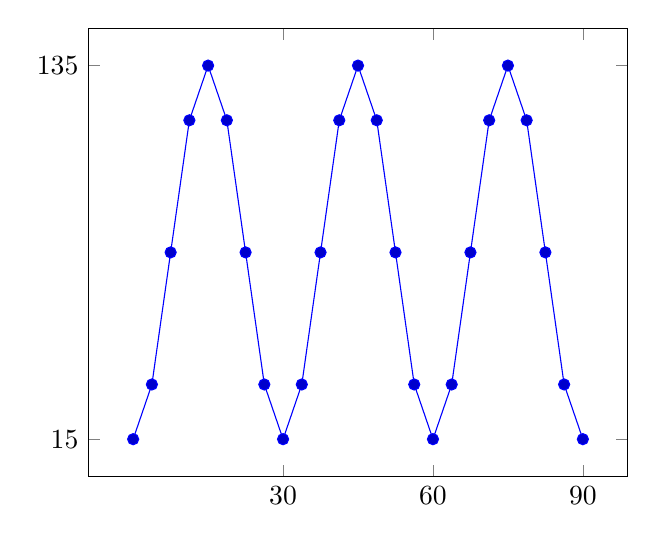
\begin{tikzpicture}
        \begin{axis}[xtick={30, 60, 90}, ytick={15, 135}]
          \addplot+[domain=0:90] {-60*cos(deg(pi/15*x))+75};
        \end{axis}
      \end{tikzpicture}
    \end{center}
    \end{solution}

    \item 
    \begin{problem}
        Determine the amplitude, midline, and period.
    \end{problem}
    \pspace{\vfill}

    \item 
    \begin{problem}
        What transformations would we need to do to either sine or cosine to get the graph of $y=h(t)$?
    \end{problem}
    \pspace{\vfill}
    
  \item
    \begin{problem}
      Write a formula for $h(t)$.
    \end{problem}
    \pspace{\vfill}

    \begin{solution}
      The graph we sketched has amplitude $60$, midline $y=75$, and
    period $30$.  Since it has a local minimum at $t = 0$, it seems
    easiest to start with $y = - \cos t$; we can then stretch this
    vertically by a factor of $60$ (to get the right amplitude), stretch
    it horizontally by a factor of $\frac{2\pi}{30}$ (to get the right
    period), and move it up by $75$ (to get the right midline value).
    This gives $\boxed{h(t) = -60\cos\left(\frac{\pi}{15}t \right)
      +75}$.

    \checkmark
      Let's check by plugging in a couple of values of $t$.  When $t =
      0$, $h(0) = - 60 (0) + 75 = 15$, which agrees with the fact that
      we start at height 15.  When $t = 15$, $h(15) = -60 \cos (\pi) +
      75 = 135$, which agrees with the fact that we are at the highest
      point after 15 minutes. 
    \end{solution}
  \end{enumerate}

\item 
  \note{Because we're not combining shifts and stretches, students will
    need to decide whether to use sine or cosine for these. Encourage them
    to think about what will be easier.

    Also, encourage students to get in the habit of checking their
    equations by plugging in the given points.
  }

  For each of the sinusoids below, determine the midline, amplitude,
  and period.  Then, write an equation for the sinusoid. (You'll need to
  decide whether to use sine or cosine.)

  \begin{enumerate}
  \item

    \note{You might want to ask some follow-up questions about this to
      focus on the choice of using $\sin$: what would $y = 3 \cos(2x) -
      1$ look like?  How could you tell that no vertical flip was
      necessary?}

    \begin{problem}
      \raisebox{1ex-\height}{
        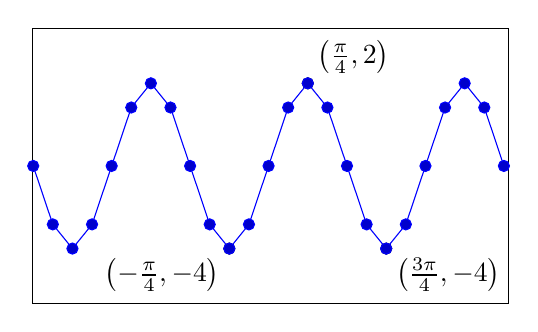
\begin{tikzpicture}
          \begin{axis}[xtick=\empty, ytick=\empty, ymin=-6, ymax=4,
            xmin=-4.72, xmax=4.8, width=3in, height=2in, clip=false]
            \addplot+[domain=-3/2*pi:3/2*pi]{3*sin(deg(2*x))-1};
            \pgfmathsetmacro\x{pi/4}; %
            \filldraw (axis cs: \x, 2) circle(2pt) node[anchor=south
            west] { $\left( \frac{\pi}{4}, 2 \right)$}; %
            \pgfmathsetmacro\y{-pi/4}; %
            \filldraw (axis cs: \y, -4) circle(2pt) node[anchor=north
            east] {$\left( - \frac{\pi}{4}, -4
              \right)$}; %
            \pgfmathsetmacro\z{3*pi/4}; %
            \filldraw (axis cs: \z, -4) circle(2pt) node[anchor=north
            west] {$\left( \frac{3\pi}{4}, -4 \right)$}; %
          \end{axis}
        \end{tikzpicture}
      }
    \end{problem}

    \begin{solution}
      To model this, it's helpful to find the
      \color{red}\emph{amplitude}\color{black},
      \color{green!70!black}\emph{midline}\color{black}, and
      \color{blue}\emph{period}\color{black}.  The amplitude is half of
      the difference between the highest value (2) and lowest value
      ($-4$), or $3$.  The midline value is the value half-way between
      $2$ and $-4$, which is $\dfrac{2 + (-4)}{2} = -1$.  The period is
      the time it takes for the graph to repeat, which we can see is
      $\pi$.  These values are shown in the picture below:
      \begin{center}
        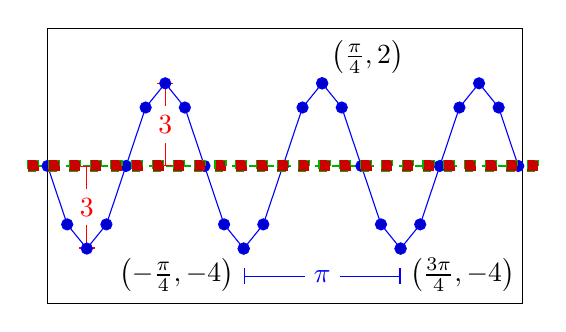
\begin{tikzpicture}
          \begin{axis}[xtick=\empty, ytick=\empty, ymin=-6, ymax=4,
            xmin=-4.72, xmax=4.8, width=3in, height=2in, clip=false]
            \addplot+[domain=-3/2*pi:3/2*pi]{3*sin(deg(2*x))-1};
            \pgfmathsetmacro\x{pi/4}; %
            \filldraw (axis cs: \x, 2) circle(2pt) node[anchor=south
            west] { $\left( \frac{\pi}{4}, 2 \right)$}; %
            \pgfmathsetmacro\y{-pi/4}; %
            \filldraw (axis cs: \y, -4) circle(2pt) node[anchor=north
            east] {$\left( - \frac{\pi}{4}, -4
              \right)$}; %
            \pgfmathsetmacro\z{3*pi/4}; %
            \filldraw (axis cs: \z, -4) circle(2pt) node[anchor=north
            west] {$\left( \frac{3\pi}{4}, -4 \right)$}; %
            \addplot+[dashed, green!70!black] { -1};
            \draw[|-|, blue] (axis cs: \y, -5) -- node[fill=white] {$\pi$} (axis
            cs: \z, -5);
            \pgfmathsetmacro\a{-3*pi/4};
            \draw[|-|, red] (axis cs: \a, 2) -- node[fill=white] {$3$}
            (axis cs: \a, -1);
            \pgfmathsetmacro\b{-5*pi/4};
            \draw[|-|, red] (axis cs: \b, -4) -- node[fill=white] {$3$}
            (axis cs: \b, -1);
          \end{axis}
        \end{tikzpicture}
      \end{center}
      Next, we should decide whether to start with $y = \sin x$ or $y =
      \cos x$ and whether we need a vertical flip.  It's generally
      easiest to look at what's happening at $x = 0$: here, our function
      is at its midline value, and it's increasing; that's the same
      behavior that $y = \sin x$ has.  So, we can get our function by
      starting with $\sin x$, stretching vertically by a factor of 3 to
      make everything 3 times as tall (to get the right amplitude),
      stretching horizontally by a factor of $\frac{1}{2}$ (to get the
      right period), and shifting down by 1 (to get the right midline
      value).  Therefore, one possible formula for the graph is
      $\boxed{y = 3\sin(2x) -1}$.\footnote{There are always infinitely
        many possible formulas for a given sinusoidal graph!}  (To
      double-check that we want $2x$, rather than $\frac{x}{2}$, as our
      input into the sine function, try plugging in $x=\frac{\pi}{4}$.)

      \checkmark
        It's a good habit to check your answer by plugging in the points
        given on the graph.  For example, if we plug $x = \frac{\pi}{4}$
        into our formula $y = 3 \sin(2x) - 1$, we get $y = 3 \sin \left(
          \frac{\pi}{2} \right) - 1 = 3 - 1 = 2$, which agrees with the
        fact that $\left( \frac{\pi}{4}, 2 \right)$ is a point on the
        graph.  Similarly, if we plug in $x = \frac{3\pi}{4}$, we get $y
        = 3 \sin \left( \frac{3 \pi}{2} \right) - 1 = -4$, which agrees
        with the fact that $\left( \frac{3 \pi}{4}, -4 \right)$ is a
        point on the graph.
    \end{solution}

  \item
    \begin{problem}
      \raisebox{1ex-\height}{
        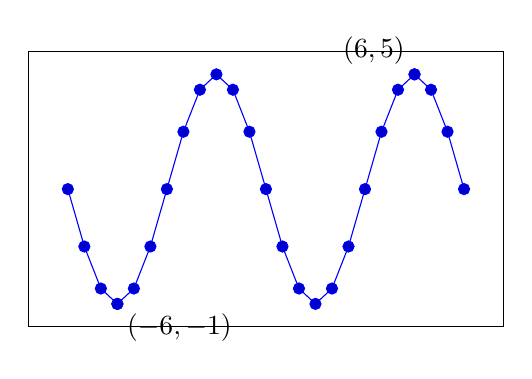
\begin{tikzpicture}
          \begin{axis}[xtick=\empty, ytick=\empty, clip=false, width=3in, height=2in]
            \addplot+[domain=-8:8]{-3*sin(deg(pi/4*x))+2};
            \filldraw (axis cs: -6, -1) circle(2pt) node[anchor=north
            west]{$(-6, -1)$};
            \filldraw (axis cs: 6, 5) circle(2pt) node[anchor=south
            east]{$(6, 5)$};
          \end{axis}
        \end{tikzpicture}
      }
    \end{problem}

    \begin{solution}
      This graph has amplitude $3$ and midline value $2$.  To figure out
      the period, it may be helpful to think in half-periods: a full
      period is the horizontal distance from one peak to the next, or
      from one trough to the next.  A half-period is therefore the
      horizontal distance from a peak to the next trough, or vice versa:
      \begin{center}
        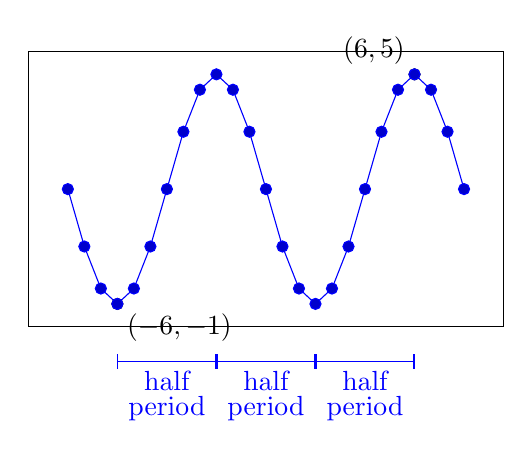
\begin{tikzpicture}
          \begin{axis}[xtick=\empty, ytick=\empty, clip=false, width=3in, height=2in]
            \addplot+[domain=-8:8]{-3*sin(deg(pi/4*x))+2};
            \filldraw (axis cs: -6, -1) circle(2pt) node[anchor=north
            west]{$(-6, -1)$};
            \filldraw (axis cs: 6, 5) circle(2pt) node[anchor=south
            east]{$(6, 5)$};
            \draw[|-|, blue] (axis cs: -6, -2.5) -- node[below,
            align=center]{half\\[-3pt] period}(axis cs: -2, -2.5); 
            \draw[|-|, blue] (axis cs: -2, -2.5) -- node[below,
            align=center]{half\\[-3pt] period}(axis cs: 2, -2.5); 
            \draw[|-|, blue] (axis cs: 2, -2.5) -- node[below,
            align=center]{half\\[-3pt] period}(axis cs: 6, -2.5); 
          \end{axis}
        \end{tikzpicture}          
      \end{center}
      So, there are 3 half-periods between $x = -6$ and $x = 6$ (a
      horizontal distance of 12 units).  That means each half period is
      4 units long, and the period is 8.

      Next, we should decide whether to start with $y = \sin x$ or $y =
      \cos x$ and whether we need a vertical flip.  At $x = 0$, our
      function is at its midline value, and it's decreasing; that's
      similar to $y = - \sin x$.  So, we can get the given graph by
      starting with $y = - \sin x$, stretching vertically by a factor of
      $3$ (to get the right amplitude), stretching horizontally by a
      factor of $\frac{8}{2 \pi} = \frac{4}{\pi}$ (to get the right
      period), and shifting up by $2$ (to get the right midline value).
      Therefore, one formula for the given function is $\boxed{y = -
        3\sin\left(\frac{\pi}{4} x\right) + 2}$.

      \checkmark
        Let's check by making sure the two points given on the graph fit
        our equation $y = - 3\sin\left(\frac{\pi}{4} x\right) + 2$.
        When $x = 6$, $y = - 3 \sin \left( \frac{3 \pi}{2} \right) + 2 =
        5$ (good!).  When $x = -6$, $y = -3 \sin \left( - \frac{3
            \pi}{2} \right) + 2 = -1$ (also good!).
    \end{solution}

  \end{enumerate}


\end{enumerate}

\end{document}